\chapter{\uppercase{Aerodynamic Database Creation}}\label{Database}

In this chapter the benefits of the proposed training and validation framework are demonstrated for an aerodynamic problem. Finally, the kriging and polynomial chaos are applied to construct aerodynamic databases of drag and lift coefficients.

\section{Flow Problem}
\label{cfdtestcase}
The steady inviscid flow around a NACA 0012 airfoil governed by the Euler equations is solved by using a second-order accurate finite-volume approach~\cite{Mani2007a,Mani2007b}.
The computational mesh is shown in Figure~\ref{mesh}.

The variations of the drag and lift coefficients with changes in Mach number ($0.5 \le$~\nom{$M_\infty$}{Mach number}~$\le 1.5$) and angle of attack ($0^{\circ} \le$ \nom{$\alpha$}{angle of attack} $\le 5^{\circ}$) are studied.
An ``exact'' database is obtained from Euler flow solves on a Cartesian mesh of $N_t=51 \times 51 = 2601$ equispaced nodes and is used to validate both the kriging and PCE surrogate models.

Figure~\ref{noise} shows the gradients obtained using a discrete-adjoint approach (demonstrated to be accurate to machine precision~\cite{Mani2007a,Mani2007b}) for two typical angles of attack,
$\alpha=1^\circ~\textrm{and}~4^\circ$. It can be seen that the gradients 
are quite noisy (due to the transonic behavior of the flux limiters) and are hence counterproductive in the construction of the surrogate models. Thus, gradients and Hessian are not used for surrogate training in this aerodynamic test case.


\begin{figure}[H]
\centering
 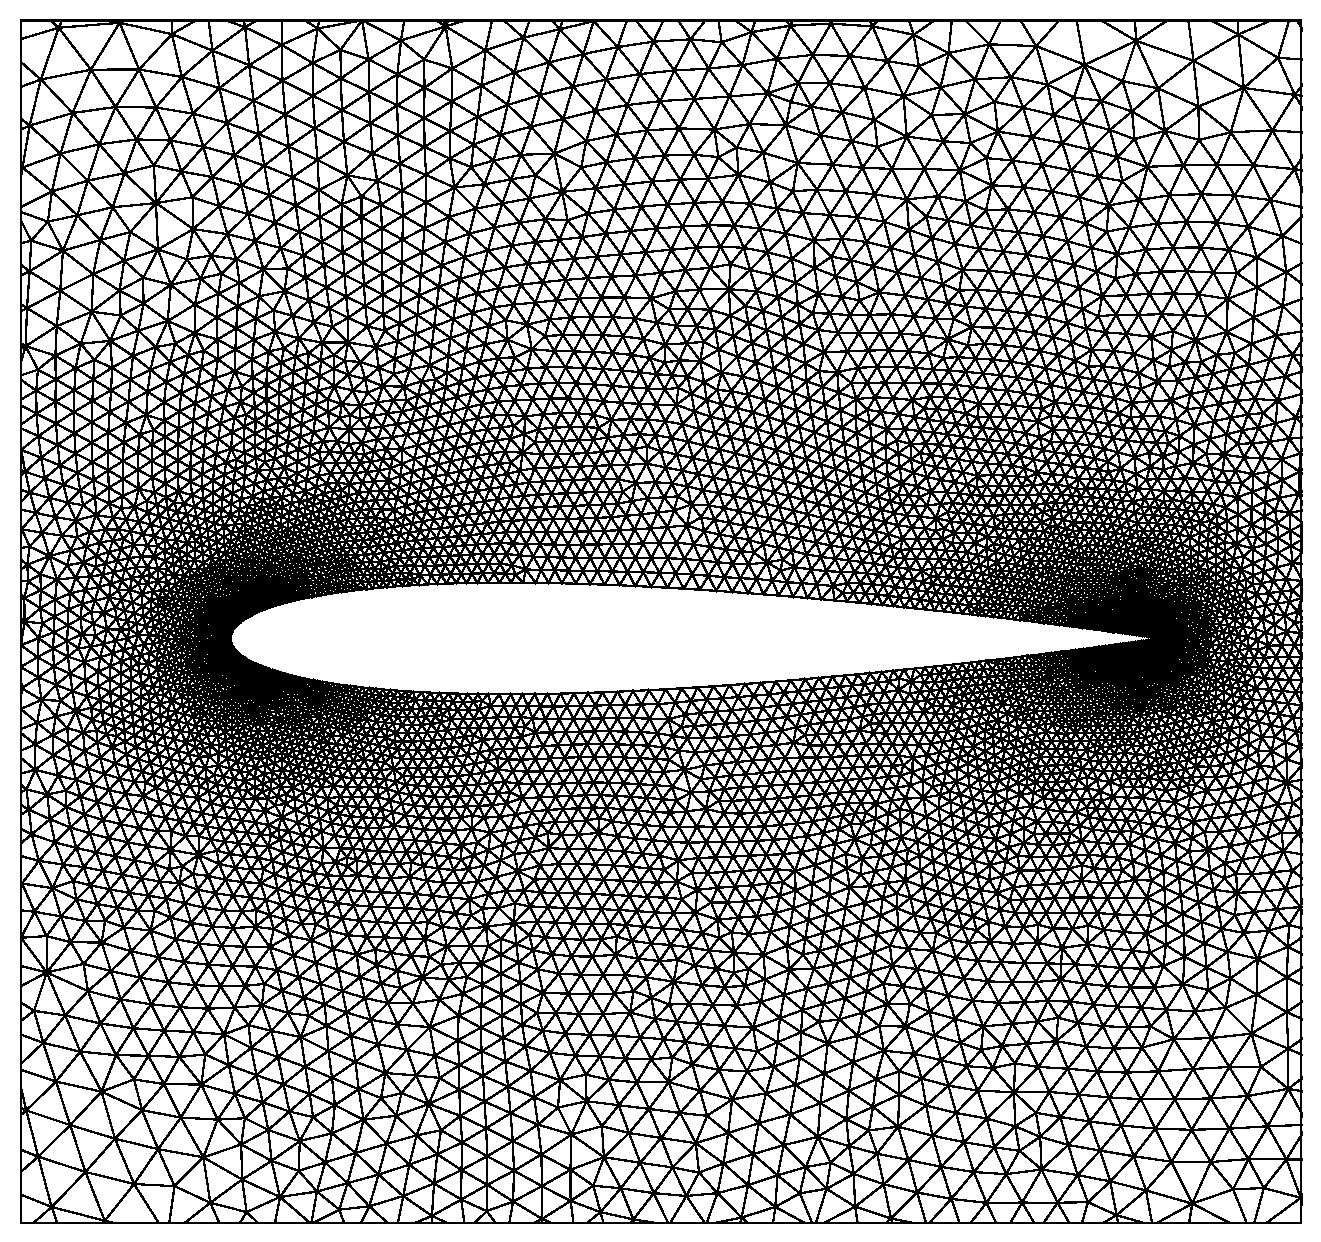
\includegraphics[width=0.45\textwidth]{finemesh.eps} 
\caption[Computational mesh for NACA 0012 airfoil.]{Computational mesh for NACA 0012 airfoil with 19,548 triangular elements.}
\label{mesh}
\end{figure}

\begin{figure}[H]
\centering
\begin{minipage}[b]{0.49\linewidth}
   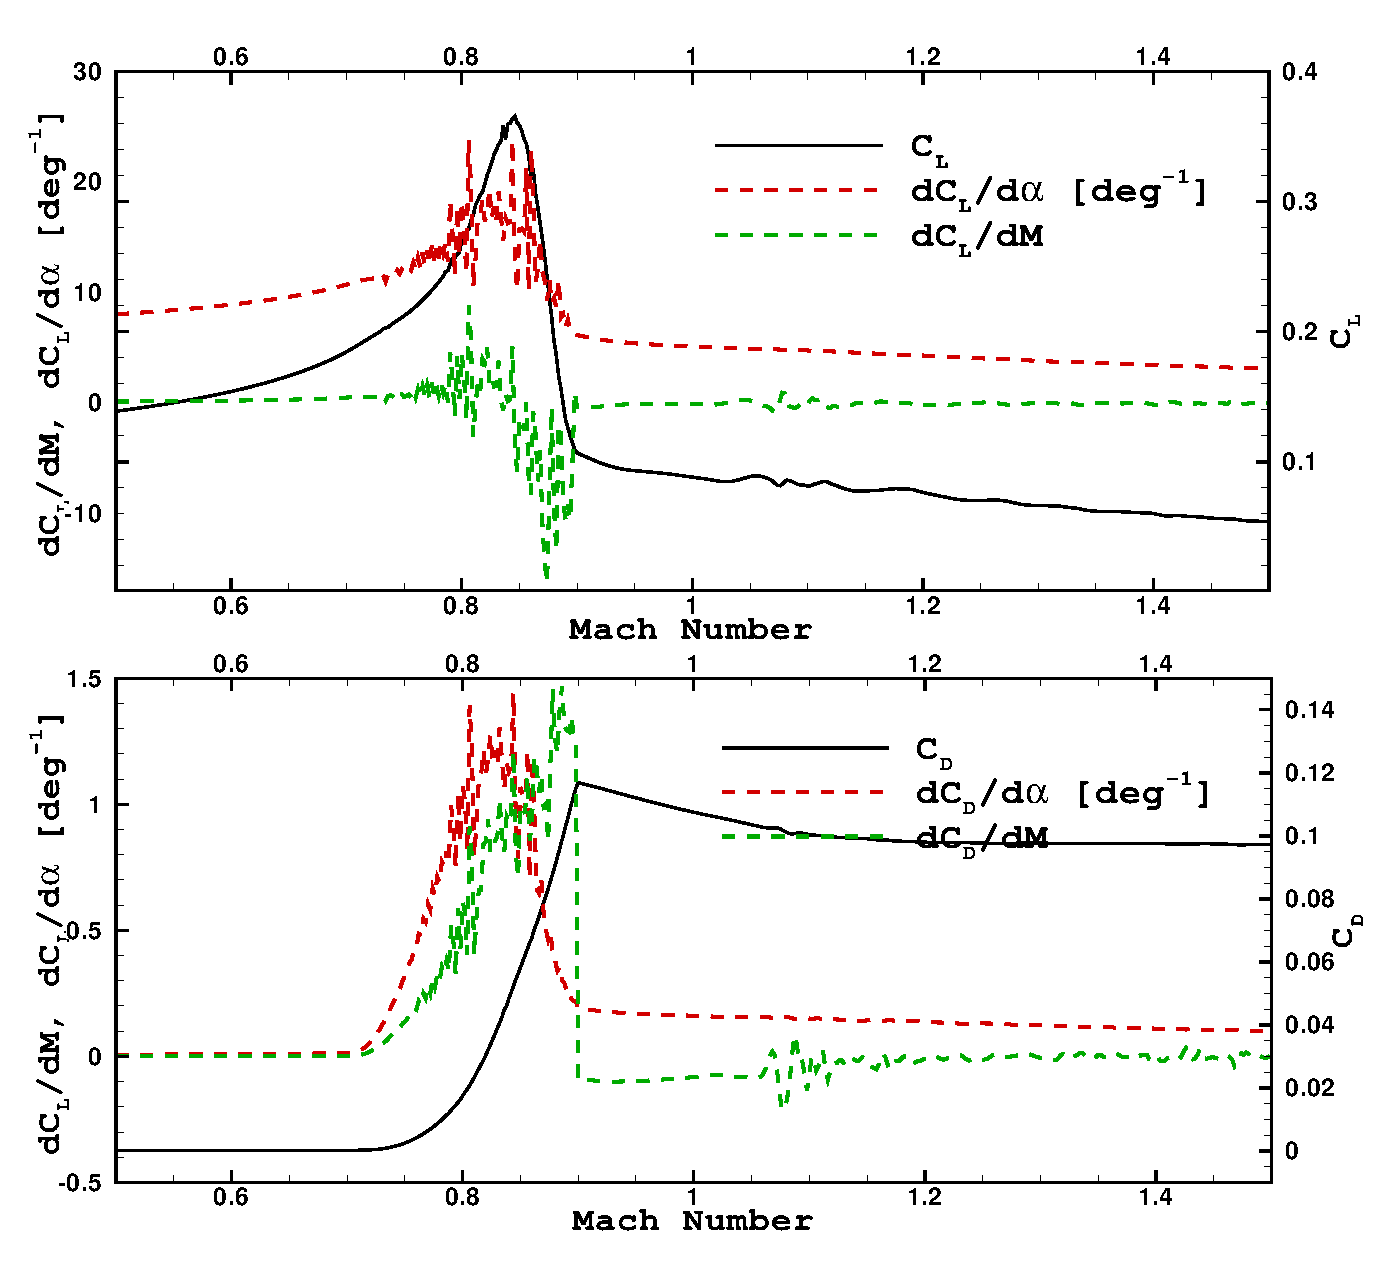
\includegraphics[width=1.0\textwidth]{alpha1.eps} 
\end{minipage}
\begin{minipage}[b]{0.49\linewidth}
  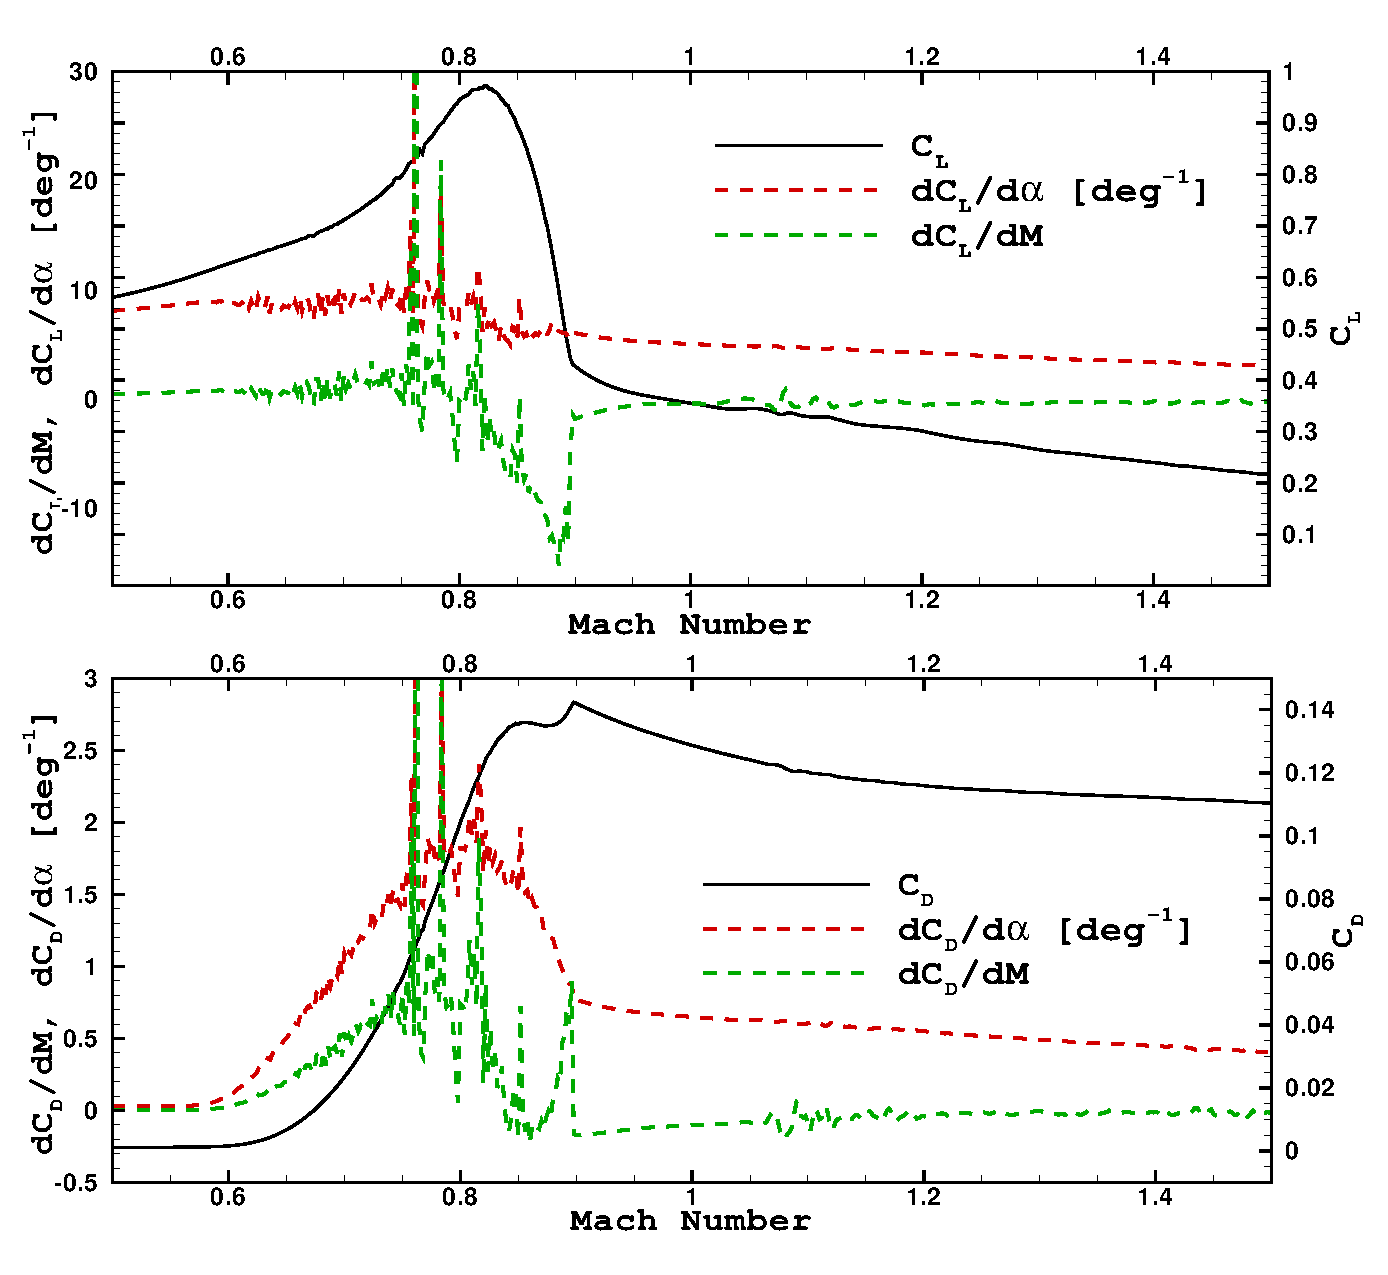
\includegraphics[width=1.0\textwidth]{alpha4.eps} 
\end{minipage}
\caption{Noisy gradients for $\alpha=1^\circ$ (left) and $\alpha=4^\circ$ (right).}
\label{noise}
\end{figure}

\section{Validation of Proposed Error Estimates}\label{rmsddemoCFD}

\subsection{Comparison with Actual Errors and Cross Validation}

\begin{figure}[h!]
\centering
\begin{minipage}[b]{0.49\linewidth}
   \includegraphics[width=1.0\textwidth]{ErrorEstimatedragkrig.eps}
\end{minipage}
\begin{minipage}[b]{0.49\linewidth}
  \includegraphics[width=1.0\textwidth]{ErrorEstimateliftkrig.eps}
\end{minipage}
\caption[Validating proposed error measures using kriging for $C_D$ and $C_L$]{A comparison of proposed error measures (blue lines) with actual errors (red lines) and leave-one-out cross validation (green lines) for drag (left) and lift coefficients (right) using kriging.}
\label{EstimateCFDKrig}
\end{figure}
\begin{figure}[h!]
\centering
\begin{minipage}[b]{0.49\linewidth}
   \includegraphics[width=1.0\textwidth]{ErrorEstimatedragPCE.eps}
\end{minipage}
\begin{minipage}[b]{0.49\linewidth}
  \includegraphics[width=1.0\textwidth]{ErrorEstimateliftPCE.eps}
\end{minipage}
\caption[Validating proposed error measures using PCE for $C_D$ and $C_L$]{A comparison of proposed error measures (blue lines) with actual errors (red lines) and leave-one-out cross validation (green lines) for drag (left) and lift coefficients (right) using PCE.}
\label{EstimateCFDPCE}
\end{figure}
In Figures~\ref{EstimateCFDKrig} and \ref{EstimateCFDPCE}, the proposed error estimates (MAD and RMSD) are compared with the actual errors (MAE and RMSE) as well as leave-one-out cross validations for kriging and PCE, respectively. 
The excellent agreement observed for analytical test functions can not be seen here. This is due to the reason that the kriging is better than MIR in approximating the non-smooth drag and lift functionals, thereby making the initial assumption 
of a more accurate local surrogate model invalid.
This opens up the avenue for exploring other candidates for building local surrogate models (e.g. radial basis function, neural networks) that can approximate non-smooth functions as good as kriging (or better).
Although not as accurate as kriging, the MIR produces reasonably accurate reference local surrogate models (see Figures~\ref{Dragdist} and ~\ref{Liftdist}).
As a result, the proposed error measures are much better in capturing the tendencies seen in global surrogate model convergence, when compared to the often used cross validation which shows misleading tendencies.

 %One could try to use better local surrogate models that can more effectively model such non-smooth functions, whose possibilities are not explored in this work. 


\subsection{Comparison with Error Distributions in the Domain}
\begin{figure}[h!]
  \centering
\begin{minipage}[b]{0.32\linewidth}
  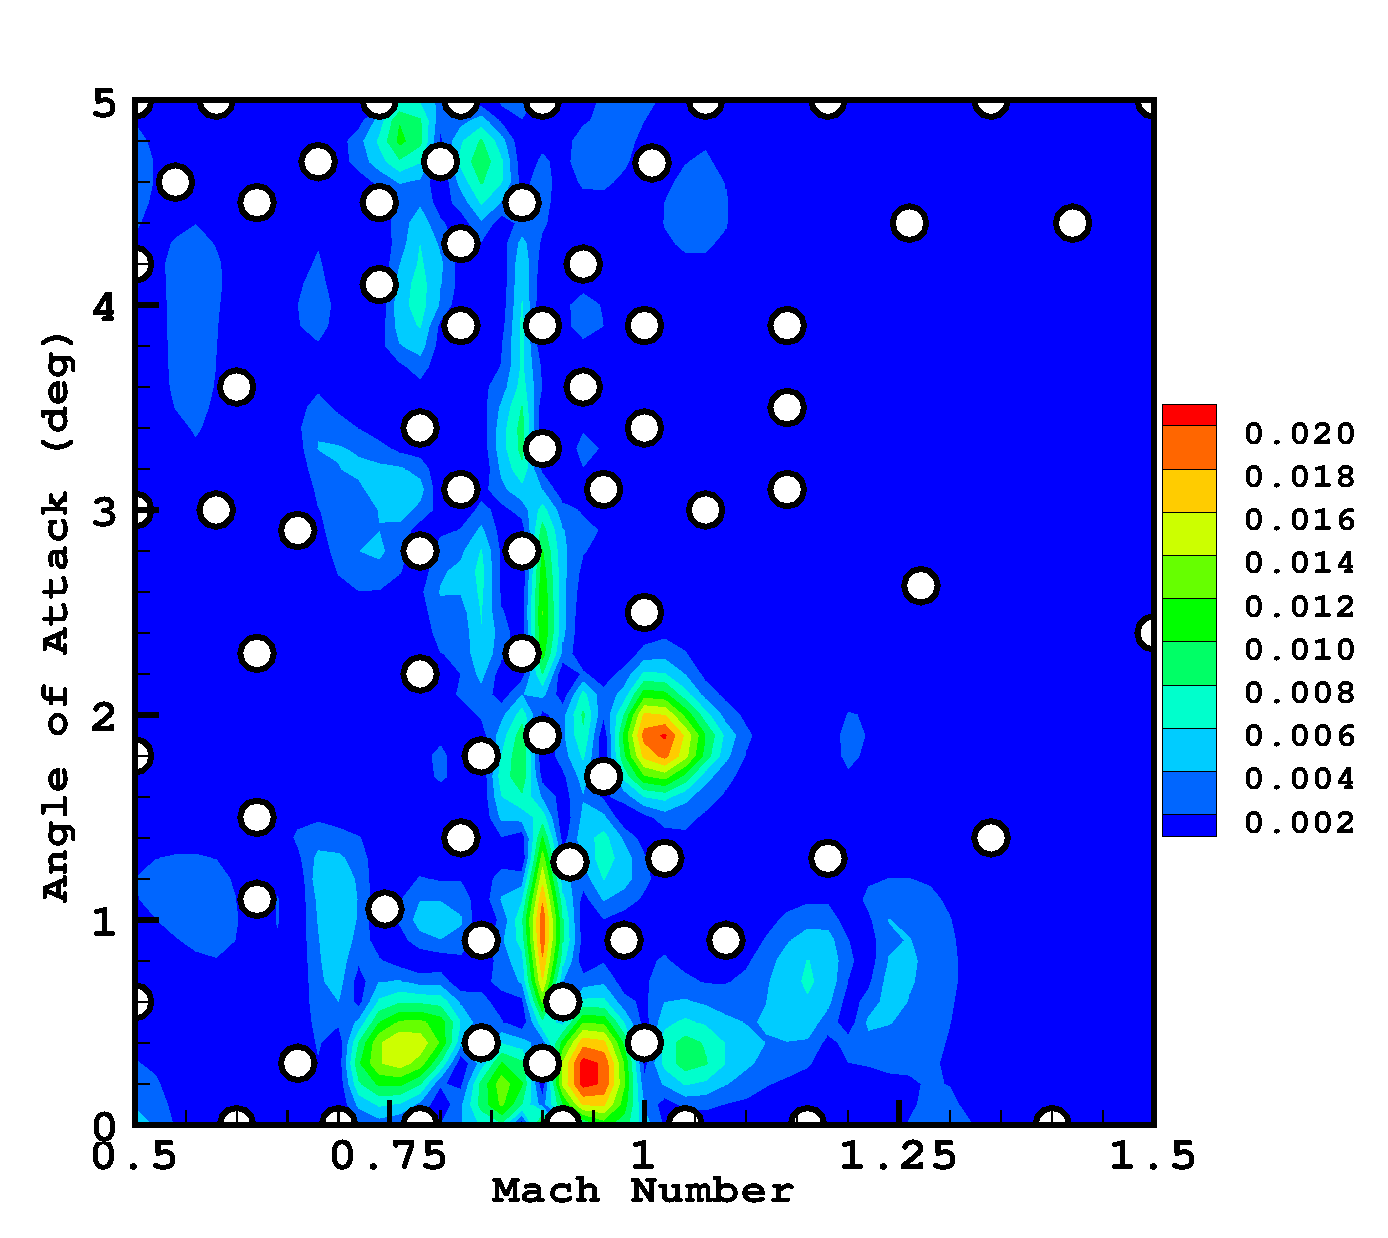
\includegraphics[width=1.0\textwidth]{MIRerrordrag75.eps} %\caption{Cosine}
\end{minipage}
\begin{minipage}[b]{0.32\linewidth}
  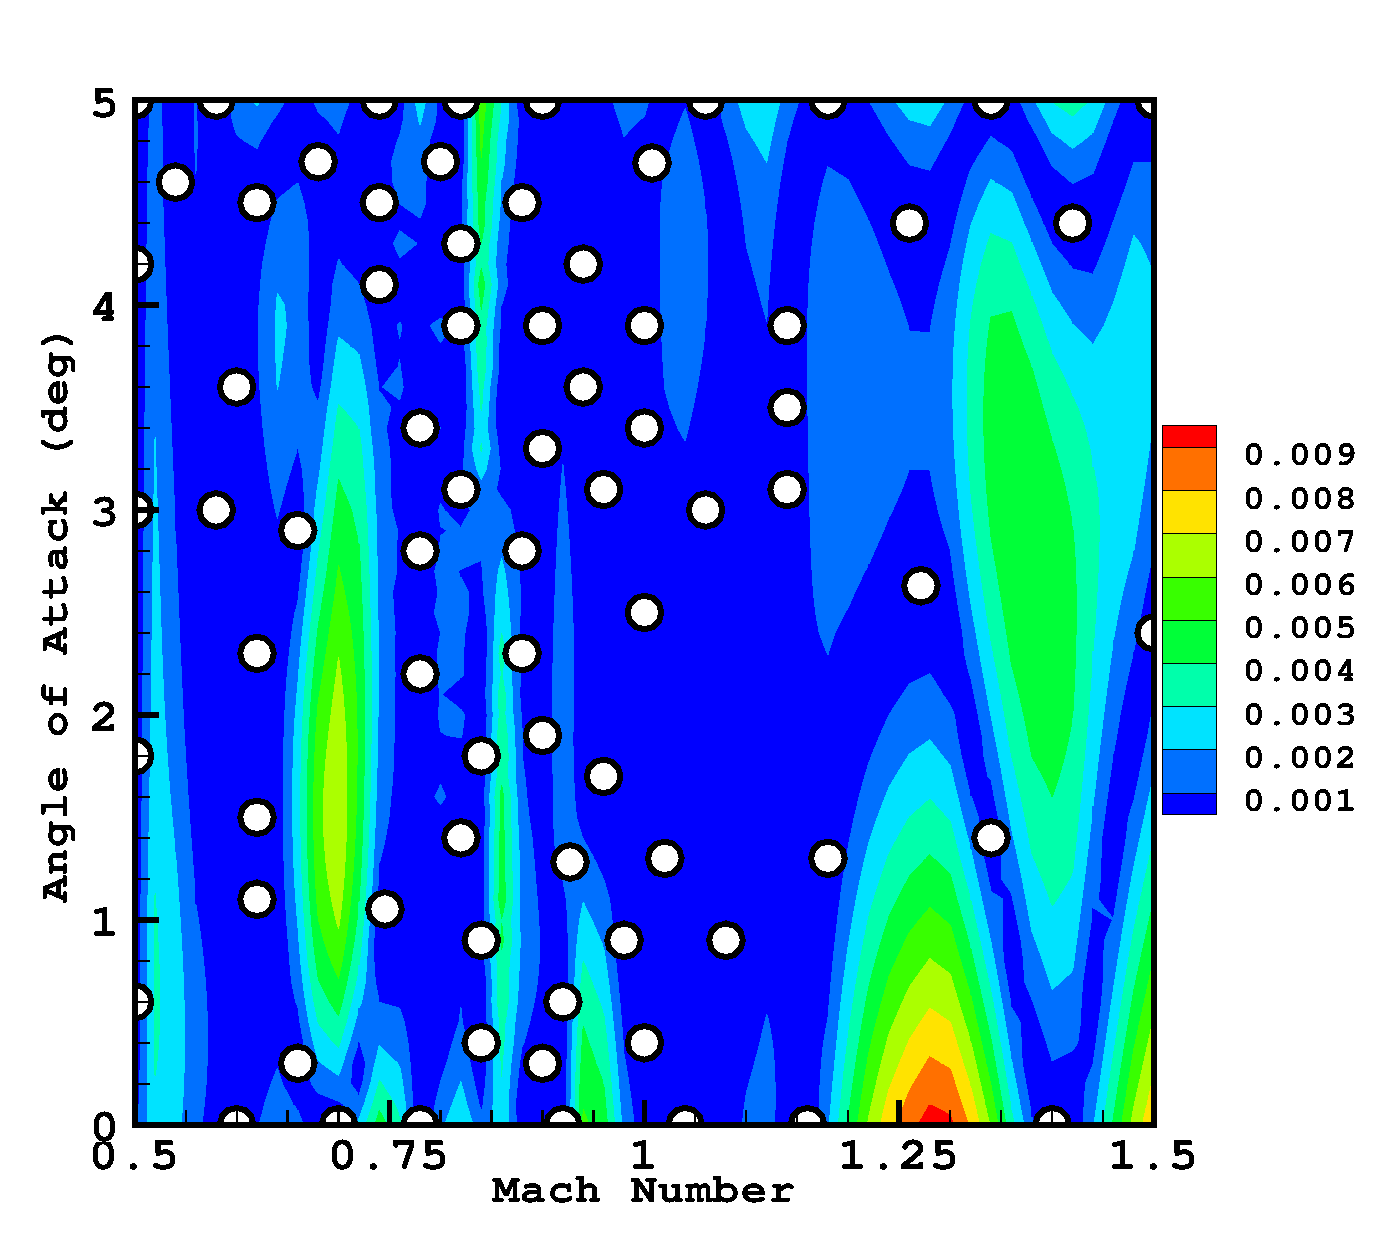
\includegraphics[width=1.0\textwidth]{rmsedrag75.eps} %\caption{Runge}
\end{minipage}
\begin{minipage}[b]{0.32\linewidth}
  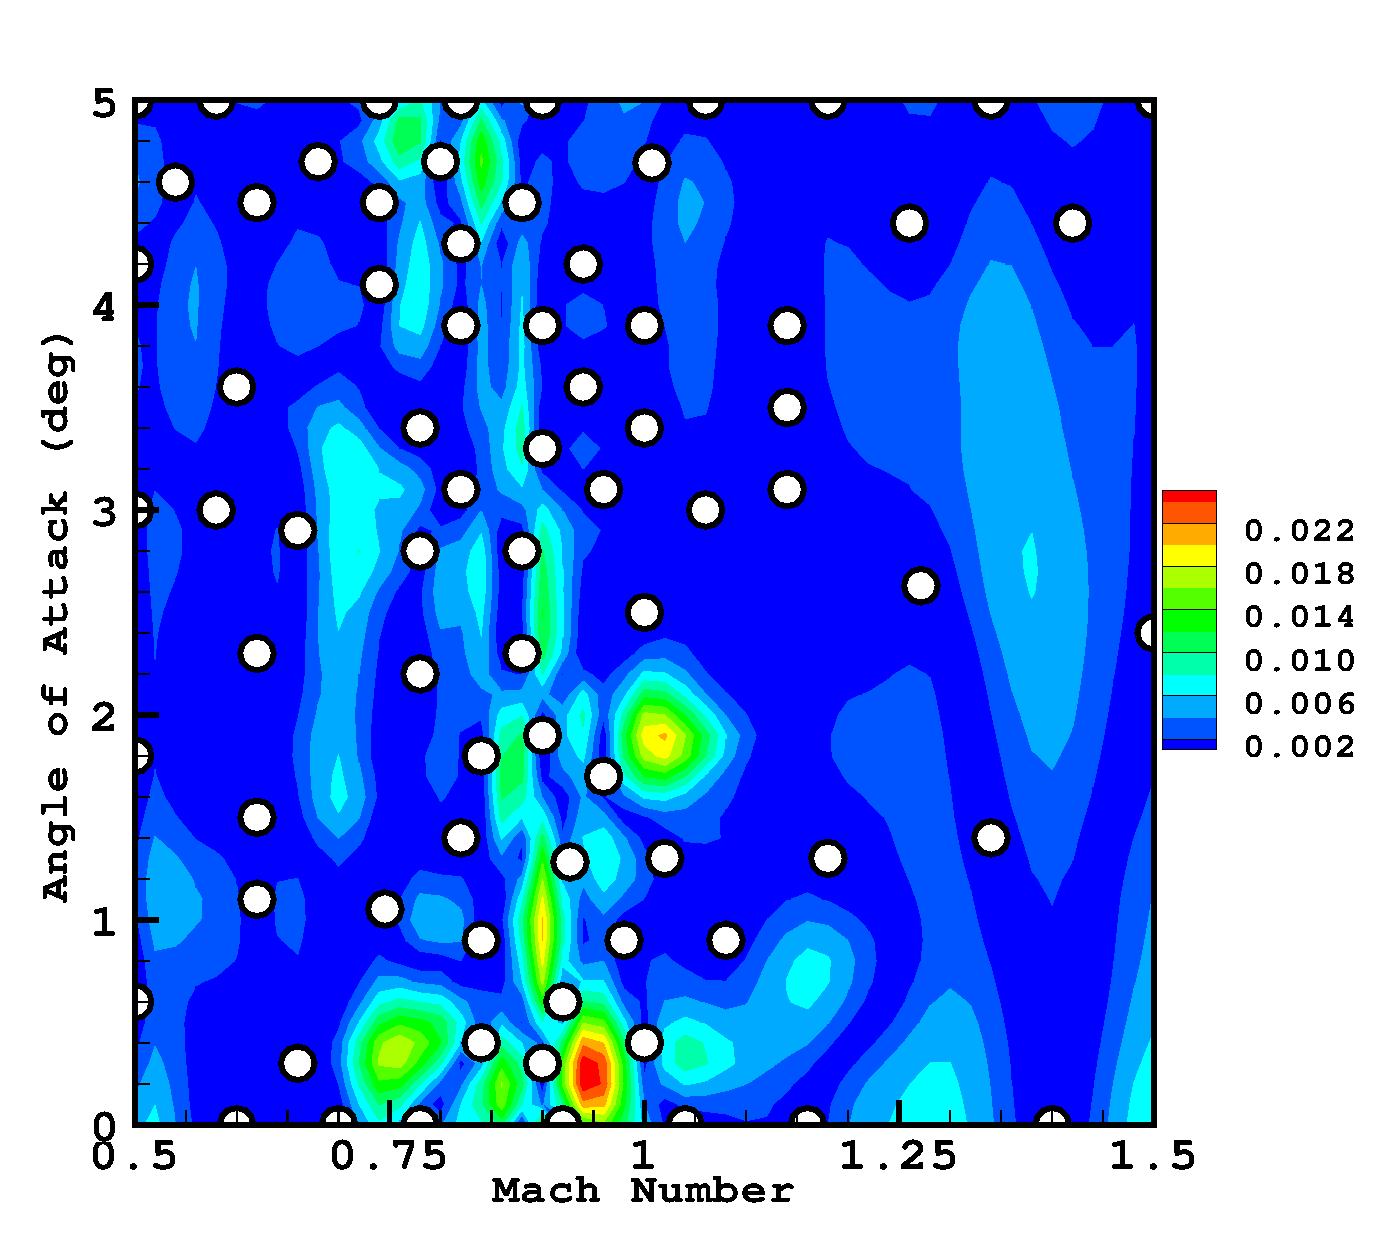
\includegraphics[width=1.0\textwidth]{rmsddrag75.eps} %\caption{Exponential}
\end{minipage}
\caption[Distribution of proposed error measures for $C_D$.]{Contour plots for the drag coefficient showing the distribution of: the local surrogate model error (left), the global kriging surrogate model error (middle) and the  proposed discrepancy function (right). The global and local surrogate models are built with 75 and 25 training points (white circles), respectively.}
\label{Dragdist}
\end{figure}
\begin{figure}[h!]
  \centering
\begin{minipage}[b]{0.32\linewidth}
  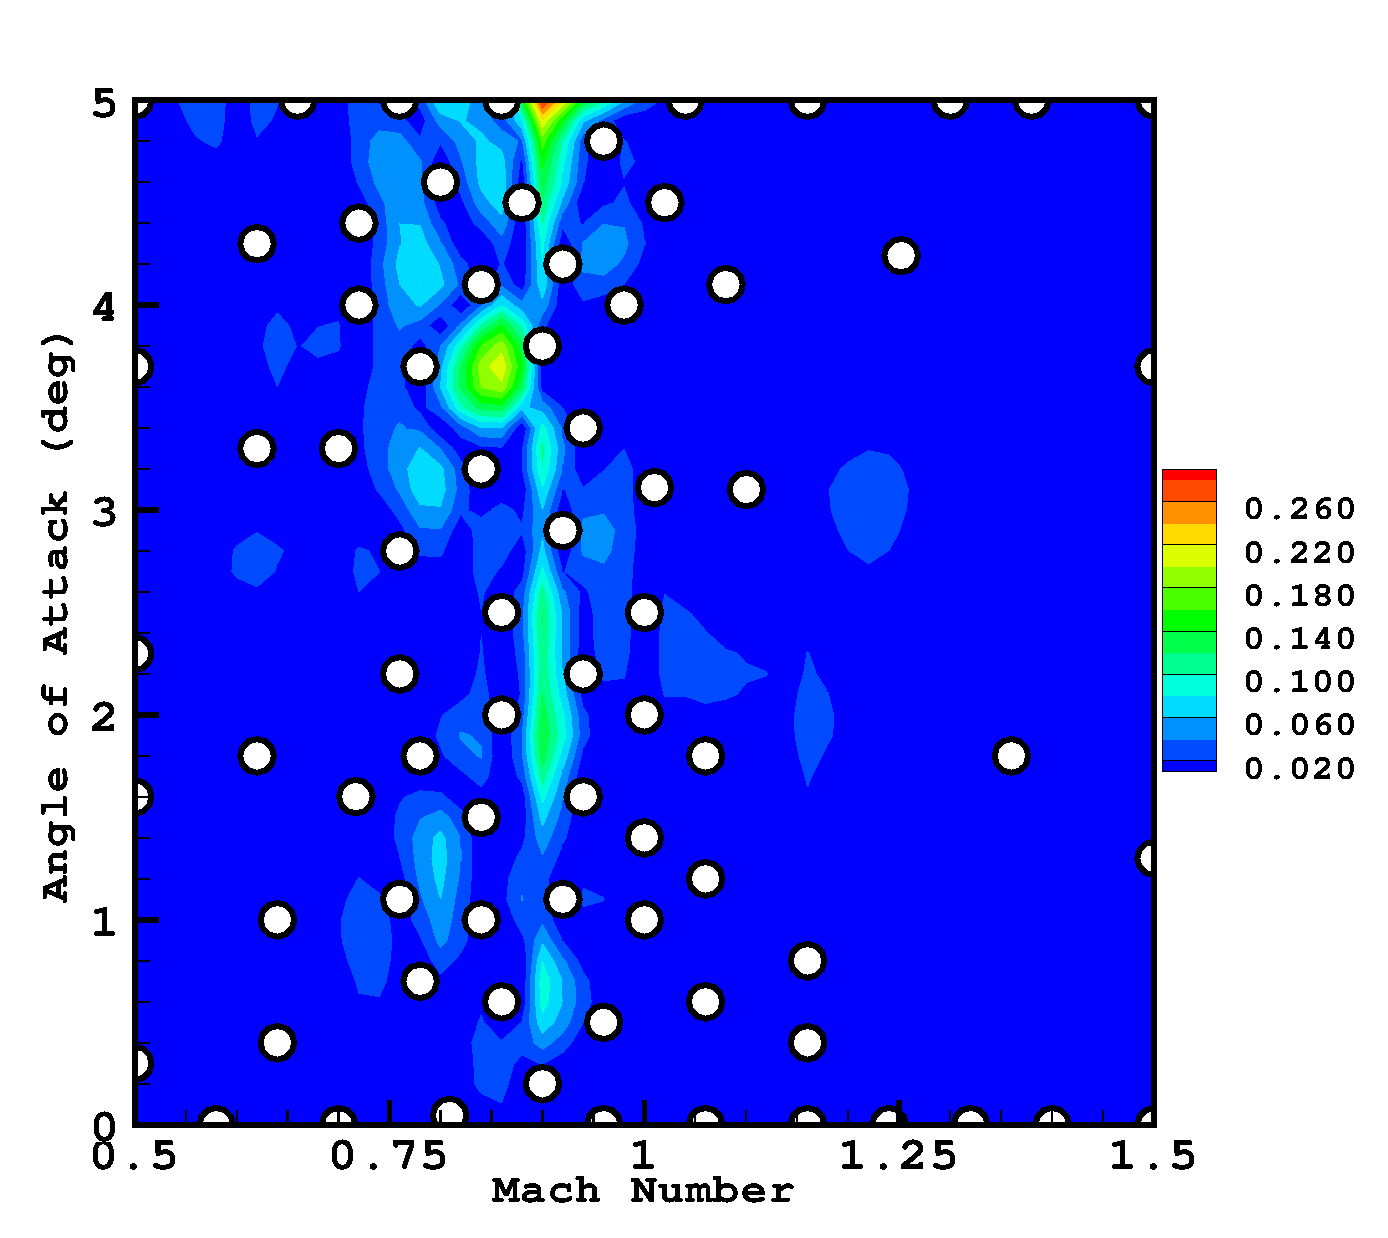
\includegraphics[width=1.0\textwidth]{MIRerrorlift75.eps} %\caption{Cosine}
\end{minipage}
\begin{minipage}[b]{0.32\linewidth}
  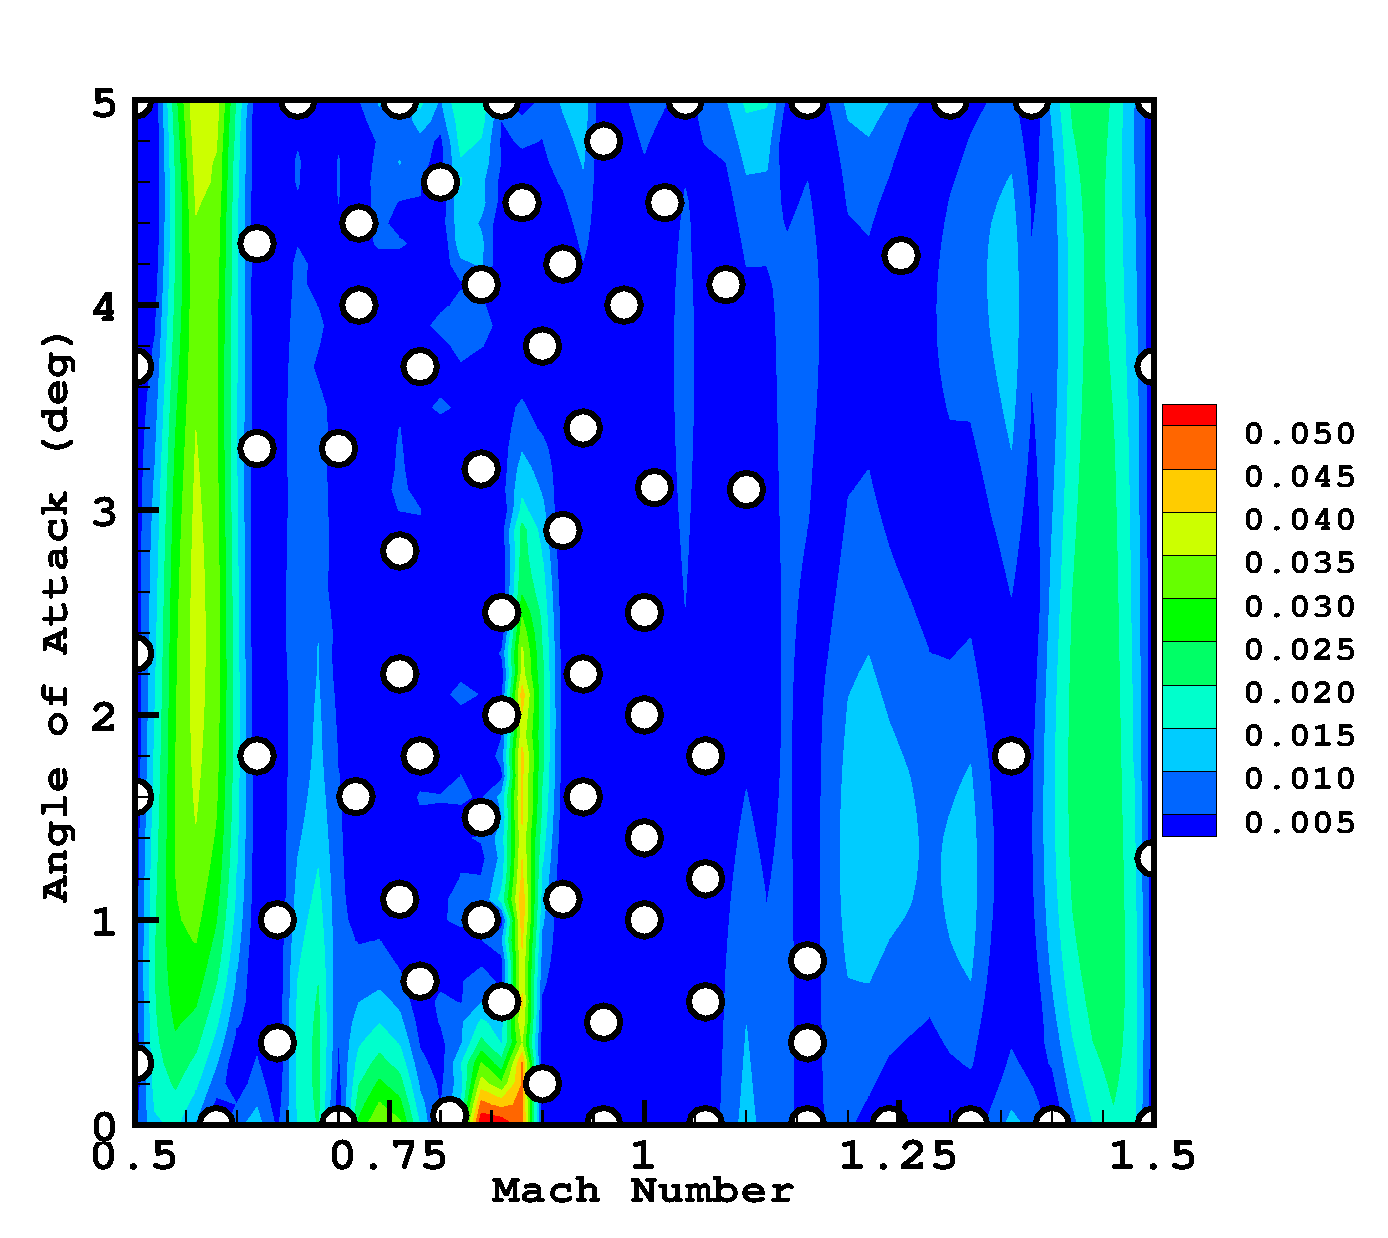
\includegraphics[width=1.0\textwidth]{rmselift75.eps} %\caption{Runge}
\end{minipage}
\begin{minipage}[b]{0.32\linewidth}
  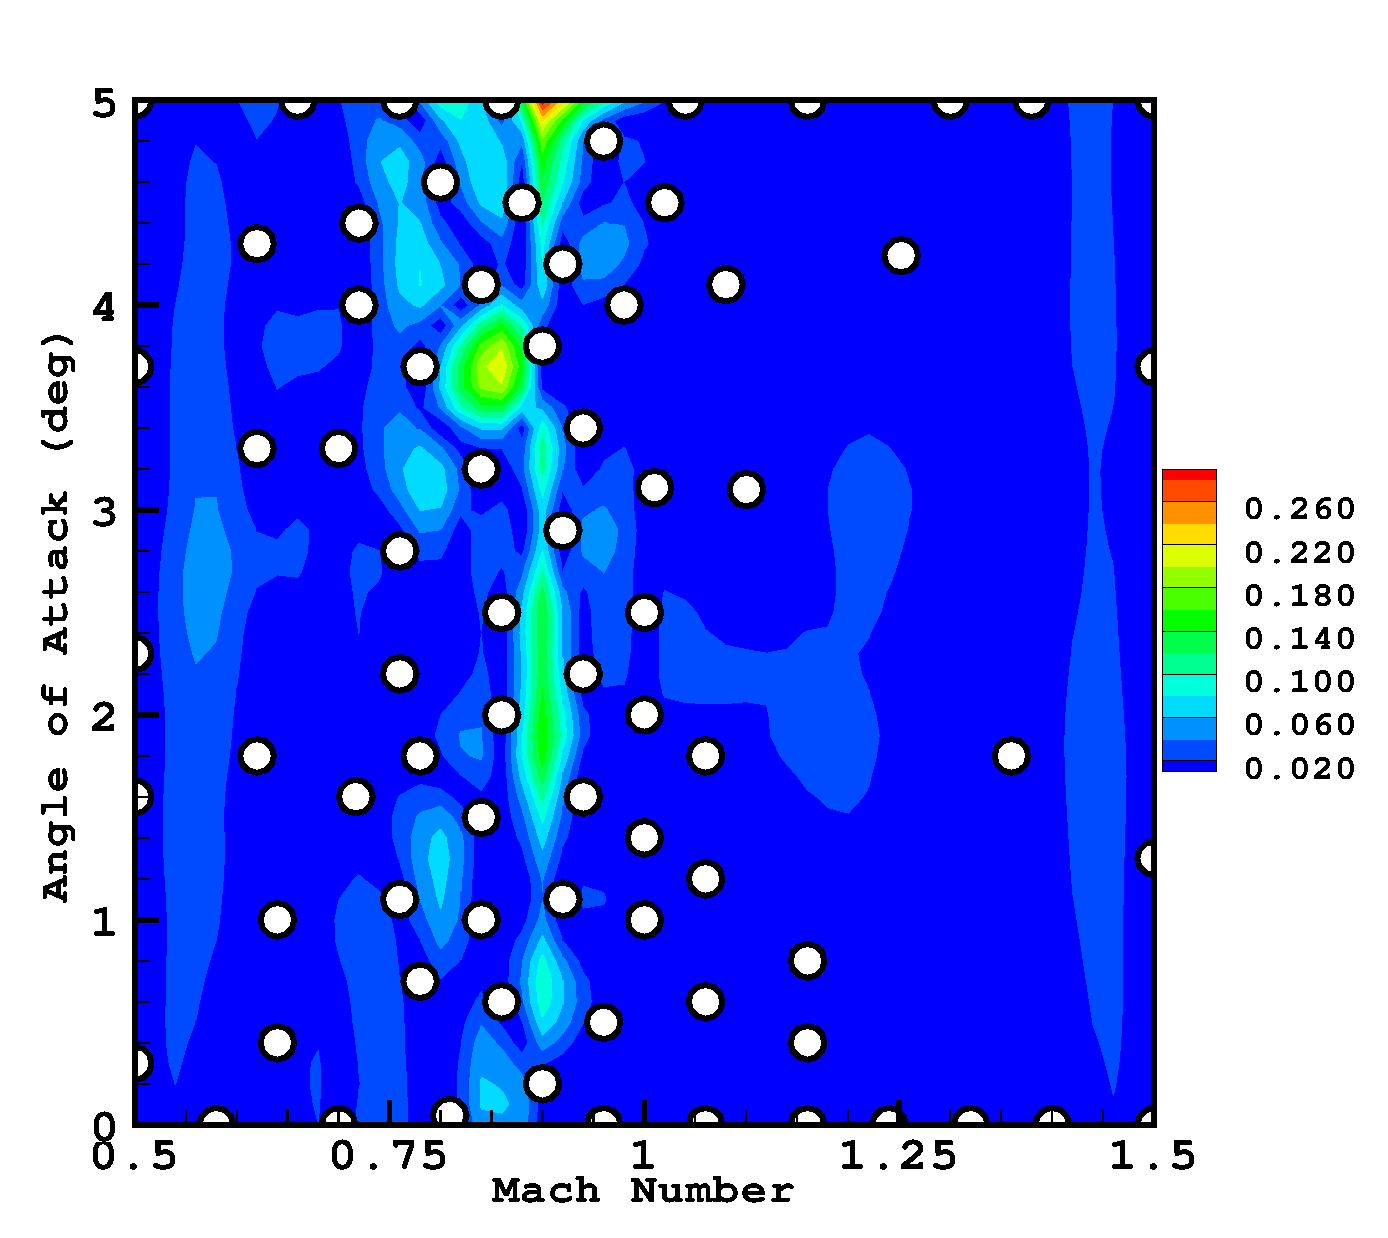
\includegraphics[width=1.0\textwidth]{rmsdlift75.eps} %\caption{Exponential}
\end{minipage}
\caption[Distribution of proposed error measures for $C_L$.]{Contour plots for the lift coefficient showing the distribution of: the local surrogate model error (left), the global kriging surrogate model error (middle) and the  proposed discrepancy function (right). The global and local surrogate models are built with 75 and 25 training points (white circles), respectively.}
\label{Liftdist}
\end{figure}
Figures~\ref{Dragdist} and ~\ref{Liftdist} show the distribution of local (left) and global surrogate model error (middle), along with the proposed discrepancy function (right), for drag and lift coefficients, respectively, using kriging as the global surrogate model.
The regions where the actual errors are high in the global kriging model (\ie~the transonic regime) are predicted reasonably well by the discrepancy function, though the magnitudes are quite different (due to inadequate local models as mentioned above). 
By comparing the contour values of error, it can also be seen that the MIR local surrogate models are less accurate than the global kriging model for both the drag and lift coefficient.
Another observation that can be made is that the dynamic training point selection method is adding a majority of the training points in the transonic region as expected. 
The kriging MSE minimization approach would not exhibit this behavior since MSE is a measure of space filling. 
If a better spread of training points is also preferred, the \emph{control parameter} described in chapter~\ref{TPSFramework} can be set to a higher value such as $1.1$ or $1.2$, that will enforce a more strict geometric constraint, 
or the vice versa when using the framework for optimizations (not studied here).
\section{Construction of Aerodynamic Database}

\subsection{Comparing Training Point Selection Methods}

Figure~\ref{cfdrmseplot} compares the performance of the proposed dynamic training point selection with other DoE methods for kriging (left) and polynomial chaos (right), respectively. 
Here, ten separate runs are averaged and the mean, best and worst trends are shown. It can be seen that the dynamic training point selection performs better than LHS for both surrogate models and for both functionals. 
\begin{figure}[h!]
  \centering
  \begin{minipage}[b]{0.49\linewidth}
    \includegraphics[width=1.0\textwidth]{rmsecfdkrig.eps} 
  \end{minipage}
  \begin{minipage}[b]{0.49\linewidth}
    \includegraphics[width=1.0\textwidth]{rmsecfdpc.eps} 
  \end{minipage}
  \caption[Dynamic versus other methods using kriging and PCE for $C_D$ and $C_L$.]{Plot of RMSE versus the number of training points for kriging (left) and PCE (right).}
  \label{cfdrmseplot}
\end{figure}
In Figure~\ref{cfdrmseplot} (left), which corresponds to kriging, minimization of MSE is also compared with the other two methods. Though not as distinct as seen with analytical test functions, 
it can be observed that the dynamic method is consistently more monotonic and accurate than other compared methods.
From Figure~\ref{cfdrmseplot} (right), it can be noticed that the accuracy of PCE tends to deteriorate with increasing order of the expansion when LHS is used. However, the dynamic training point selection prevents the early onset of such a behavior.


\subsection{Drag and Lift Coefficient Hyper-surfaces}

Figure~\ref{databaseplots} shows the exact and surrogate based contours for both the drag and lift coefficients.  It can be inferred
that the kriging model (shown in the middle column) is in good agreement with the exact model (shown in the left column) when compared to PCE (shown in the right column) which features 
high over- and undershoots in the domain.
In addition, the kriging is able to capture the transonic behavior very well, demonstrating its ability to model non-smooth functions.
Thus, for this test case the kriging proves to be a much better surrogate model than PCE. 

\begin{figure}[h!]
\centering
\begin{minipage}[b]{0.32\linewidth}
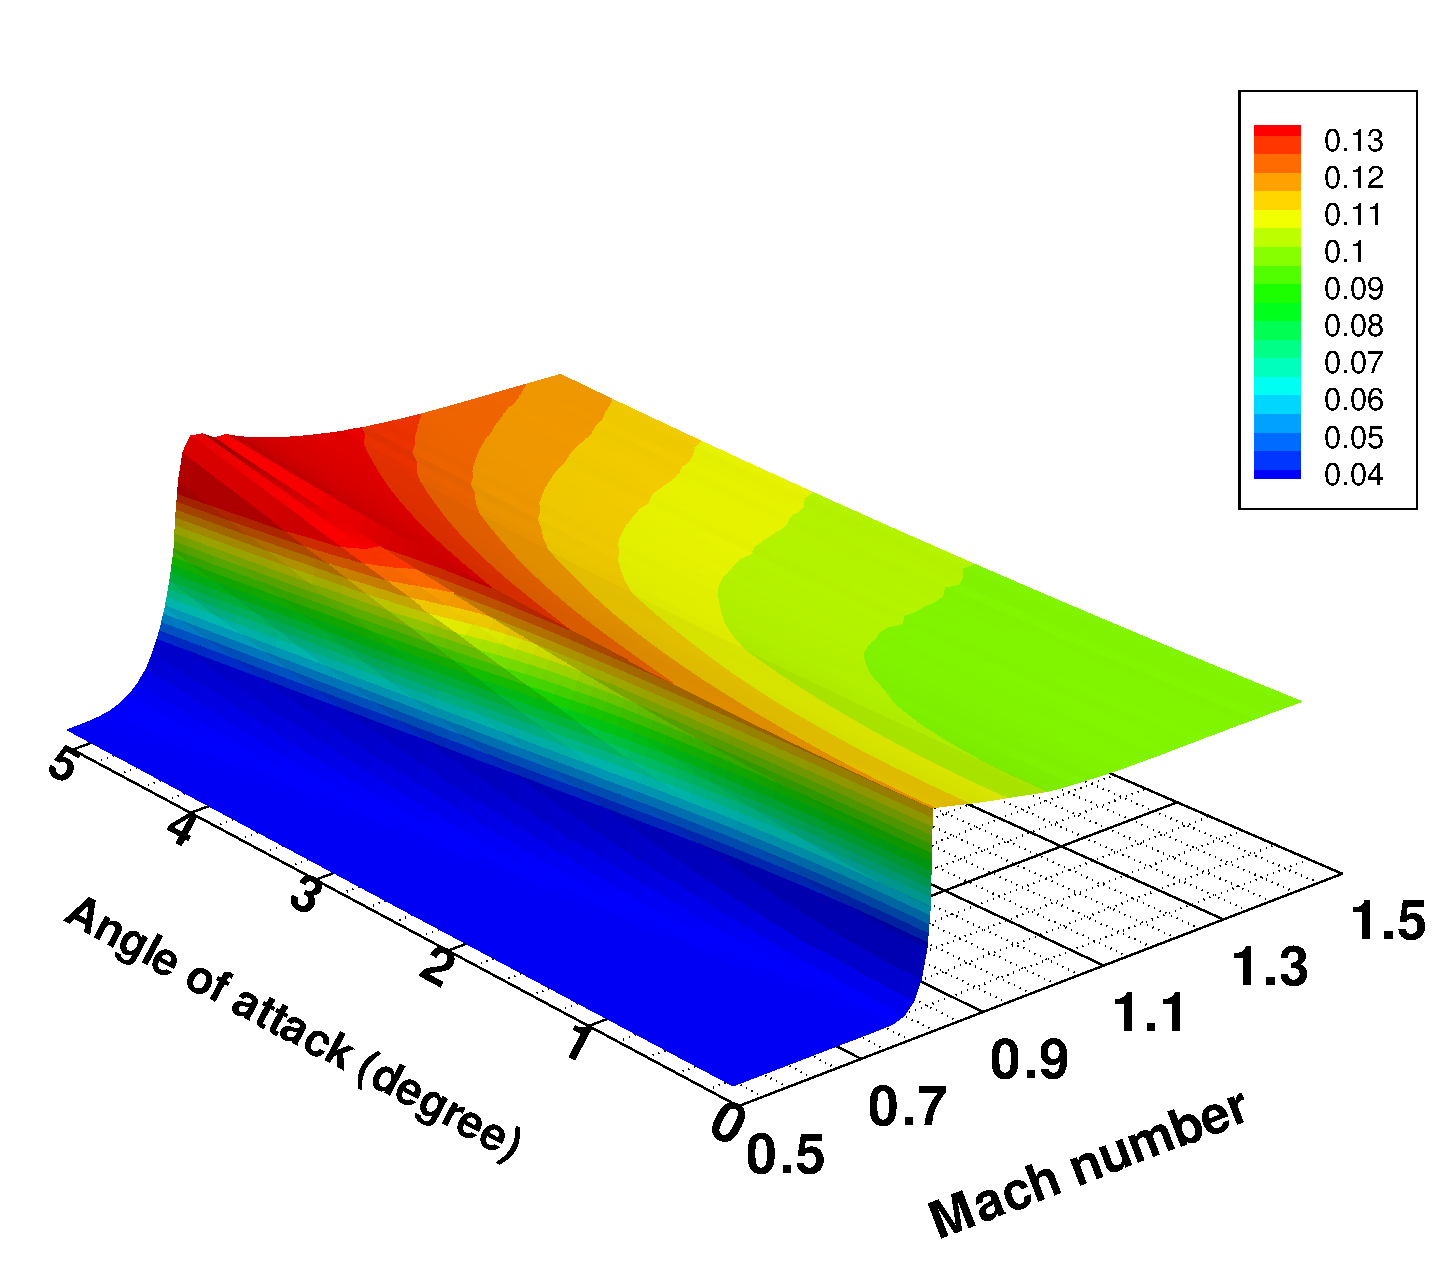
\includegraphics[width=1.0\textwidth]{dragexactonly.eps} %\caption*{Exact Drag}
\end{minipage}
\begin{minipage}[b]{0.32\linewidth}
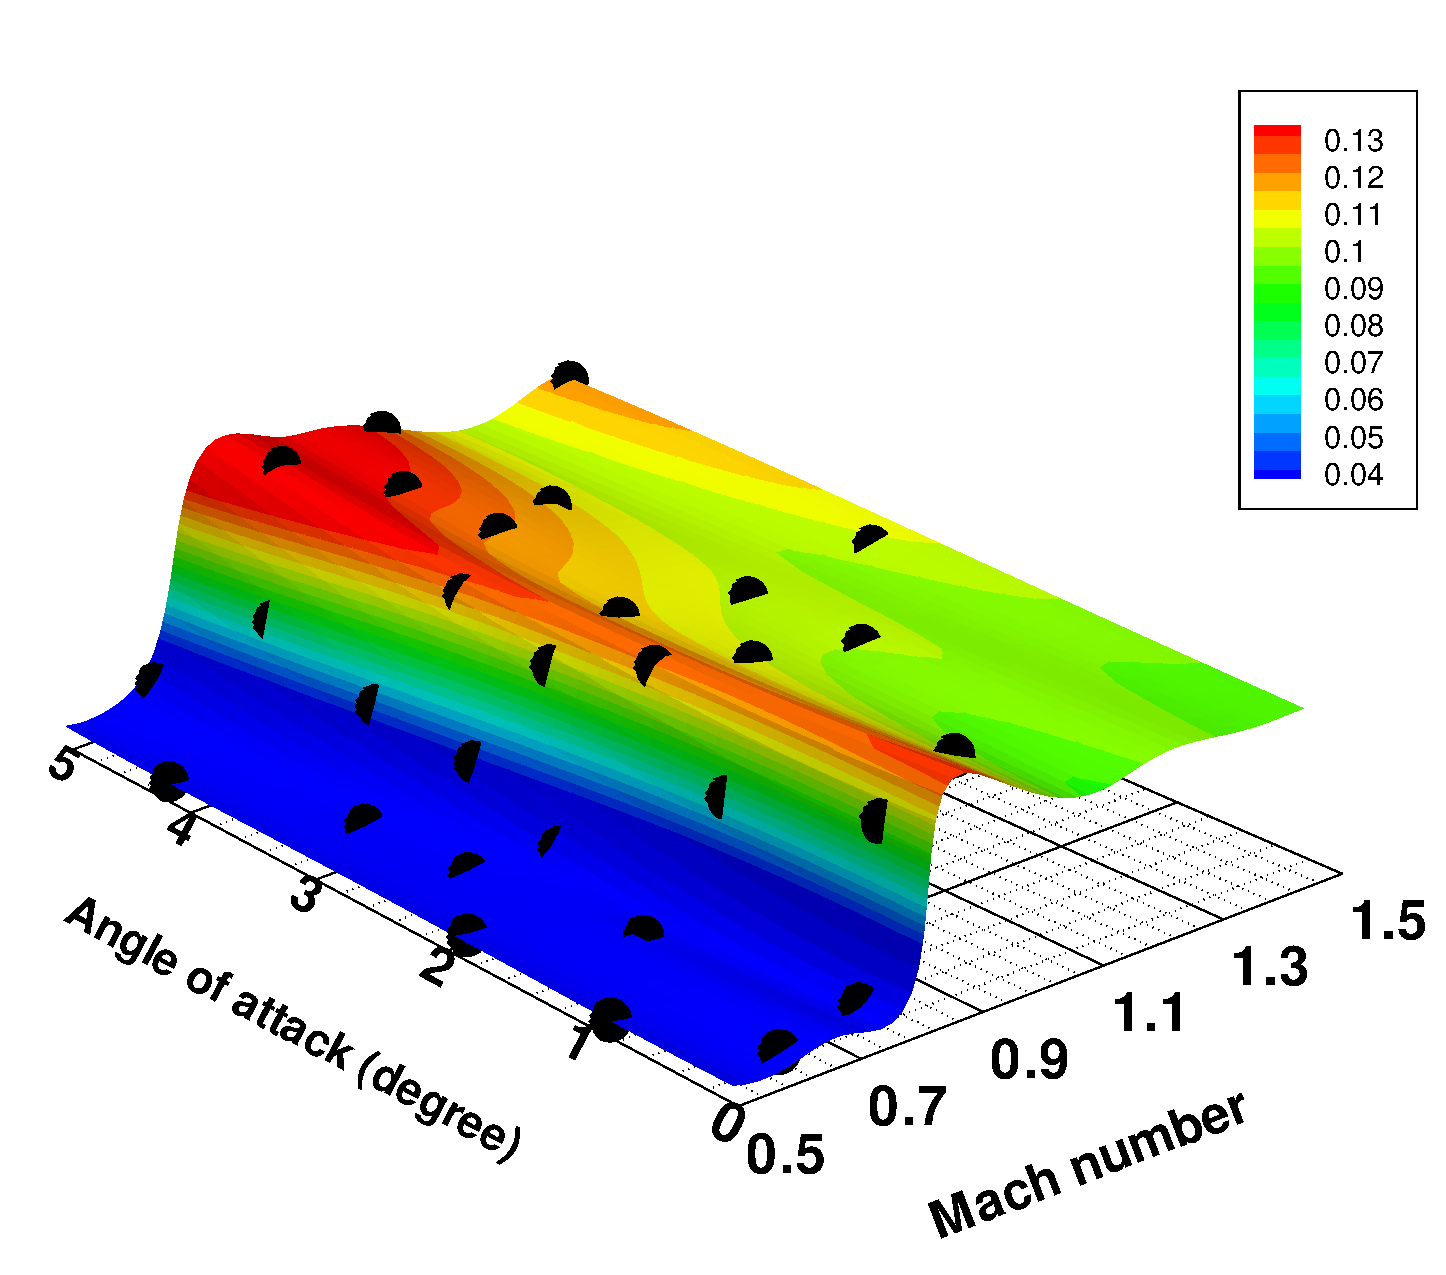
\includegraphics[width=1.0\textwidth]{krigdrag30.eps} %\caption*{Kriging Drag}
\end{minipage}
\begin{minipage}[b]{0.32\linewidth}
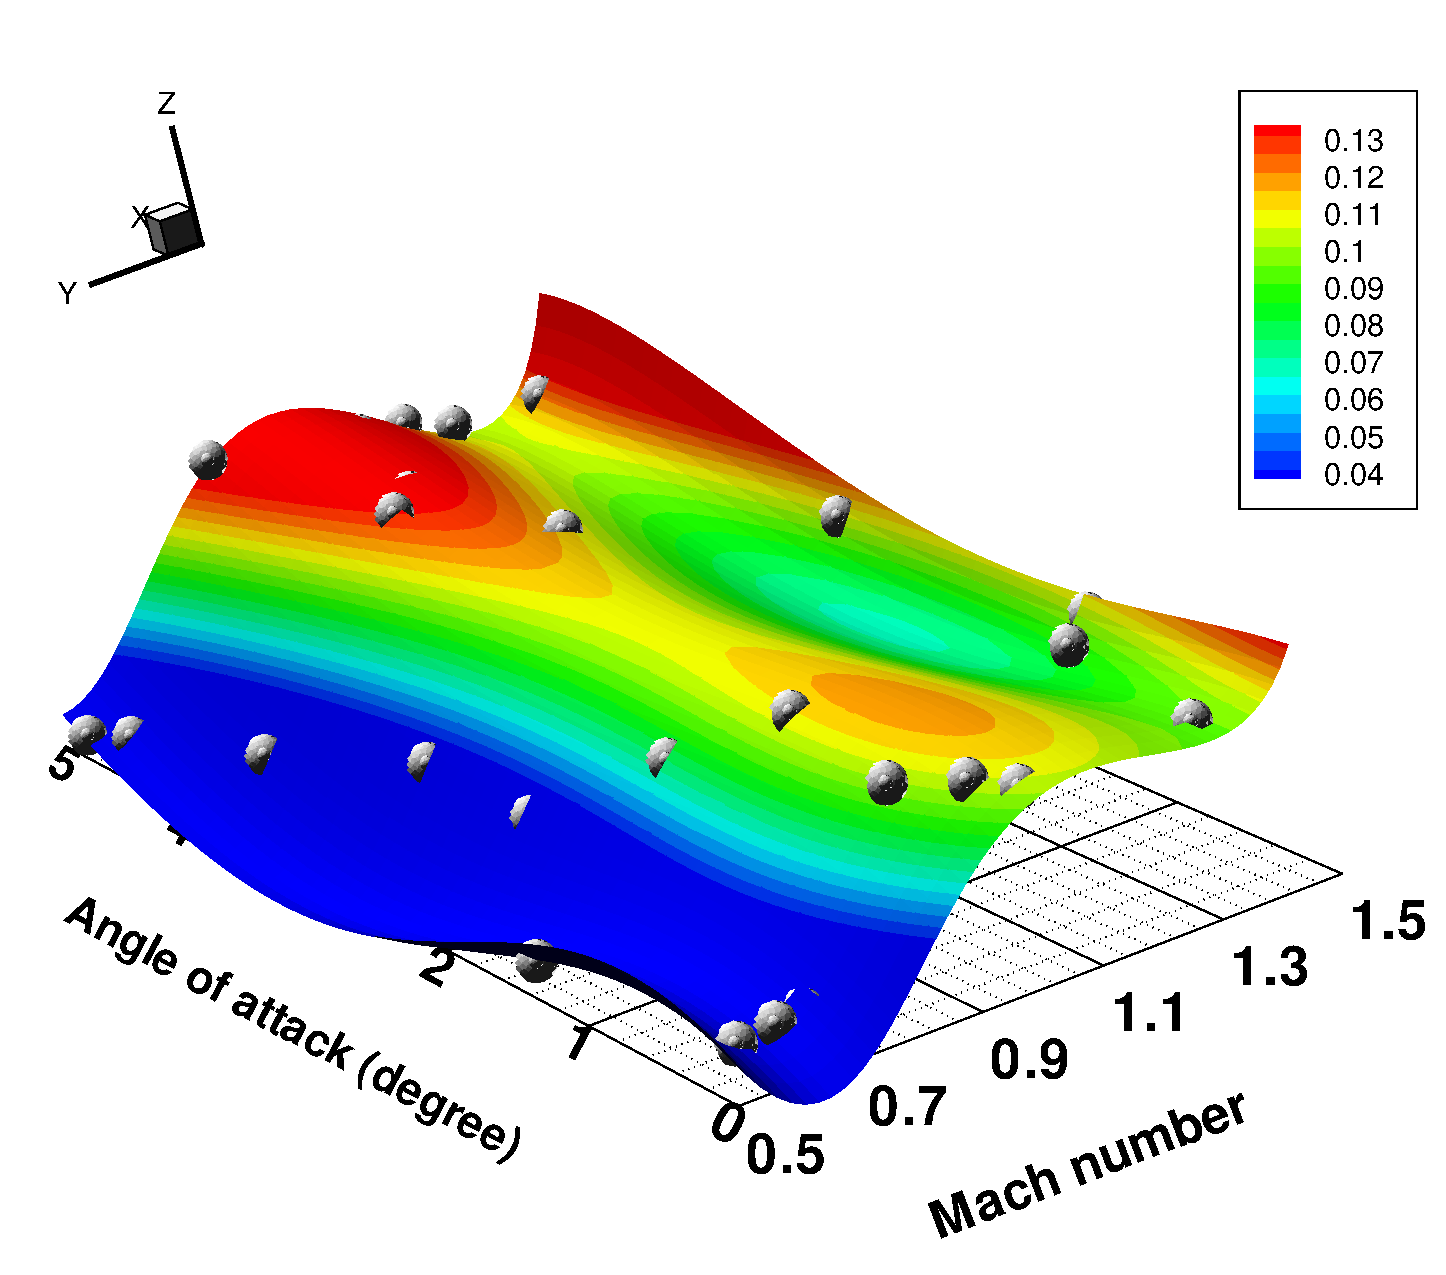
\includegraphics[width=1.0\textwidth]{dragpc30.eps} %\caption*{PC Drag}
\end{minipage}
\begin{minipage}[b]{0.32\linewidth}
   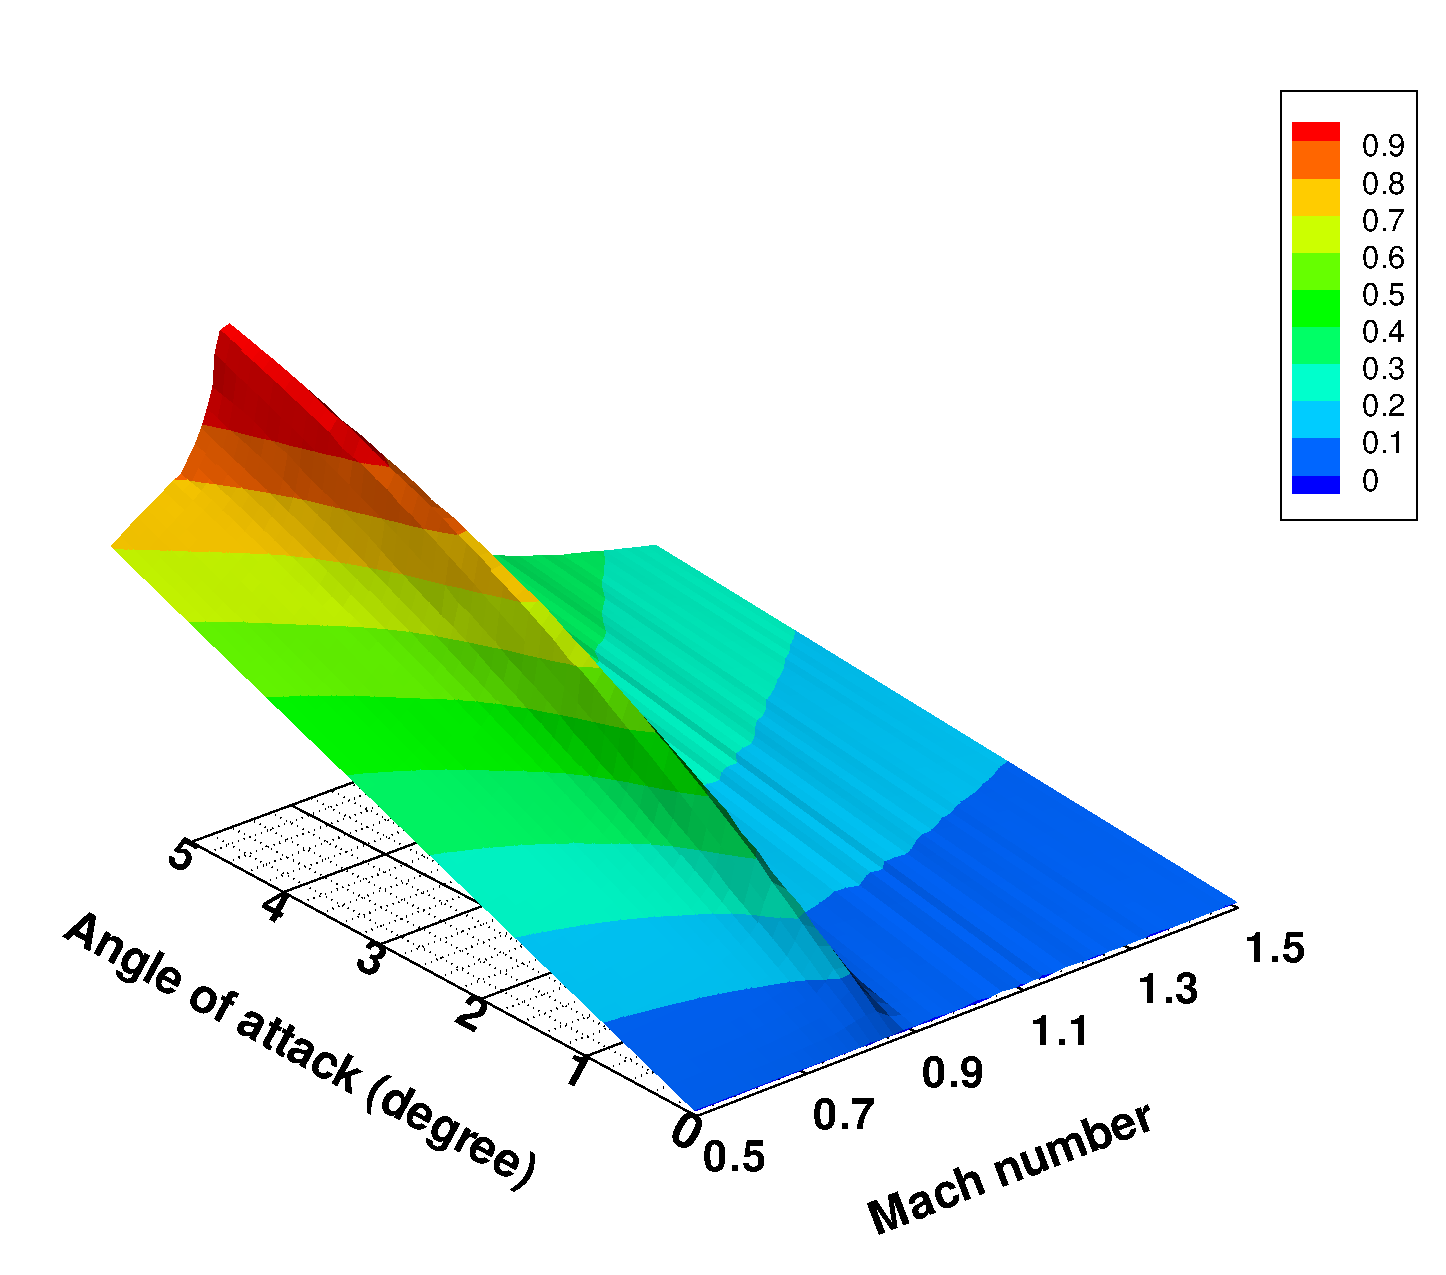
\includegraphics[width=1.0\textwidth]{liftexactonly.eps} % \caption*{Exact Lift}
\end{minipage}
\begin{minipage}[b]{0.32\linewidth}
   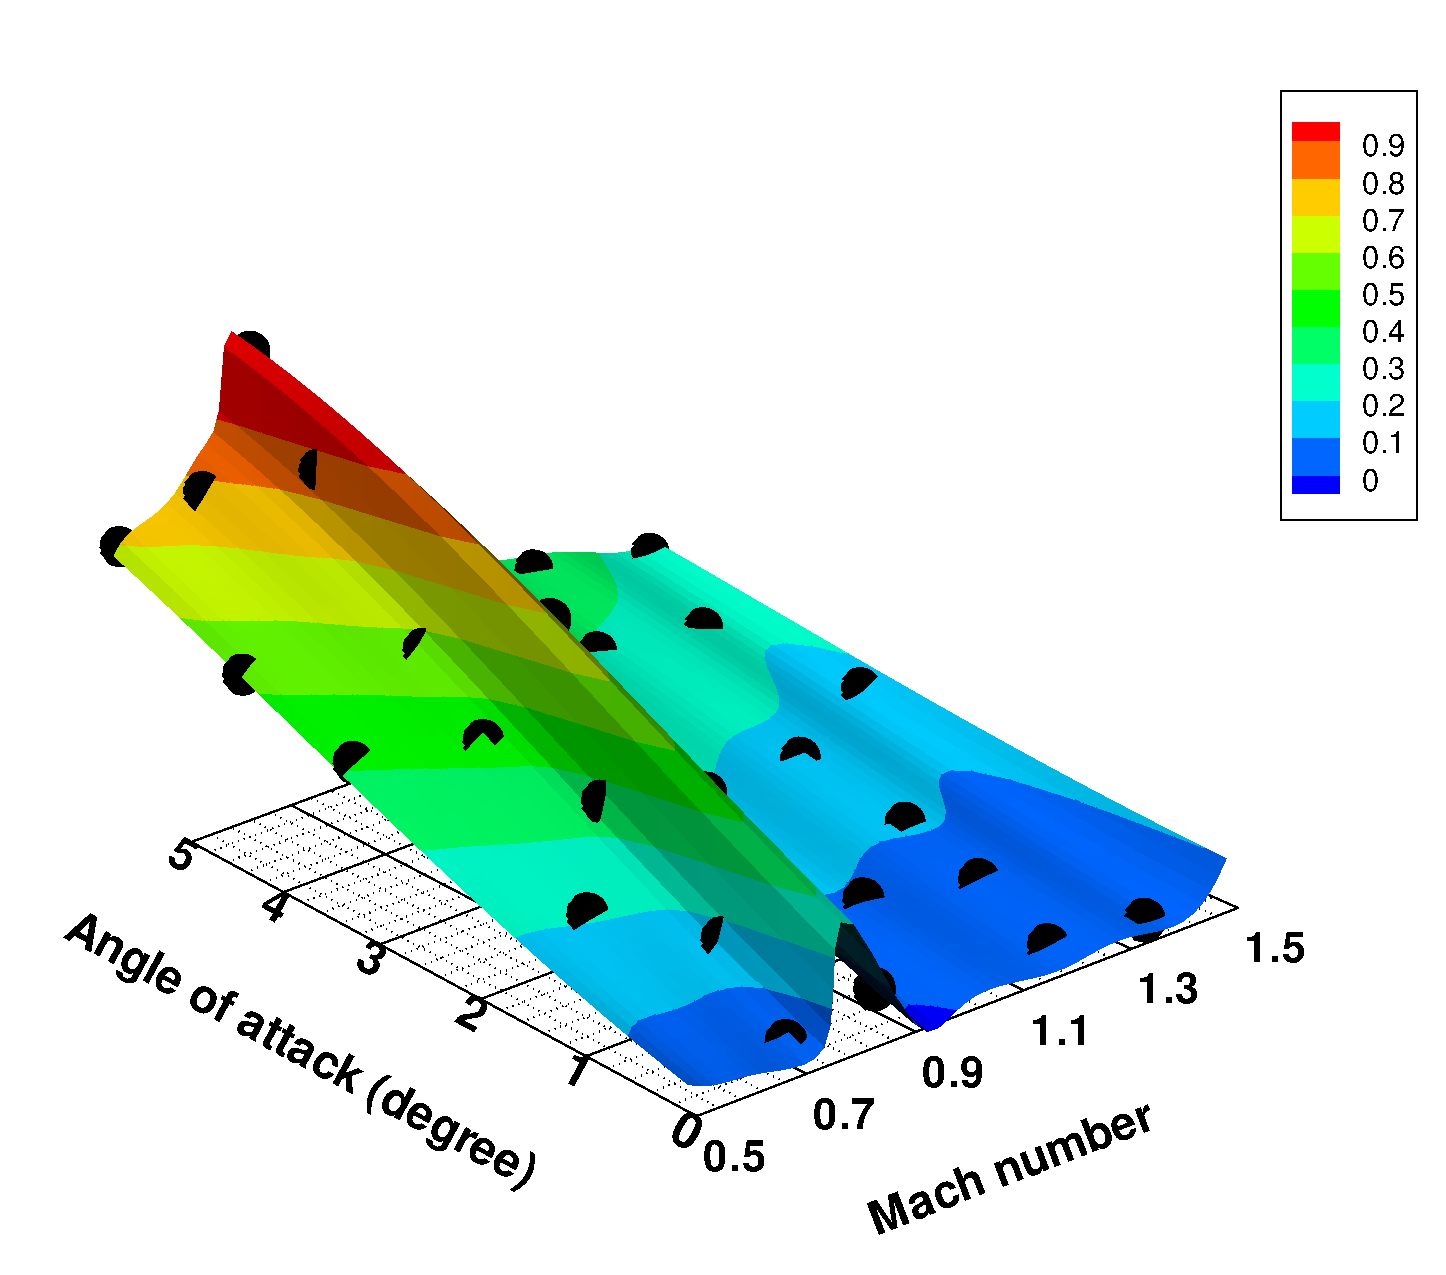
\includegraphics[width=1.0\textwidth]{kriglift30.eps}%  \caption*{Kriging Lift}
\end{minipage}
\begin{minipage}[b]{0.32\linewidth}
   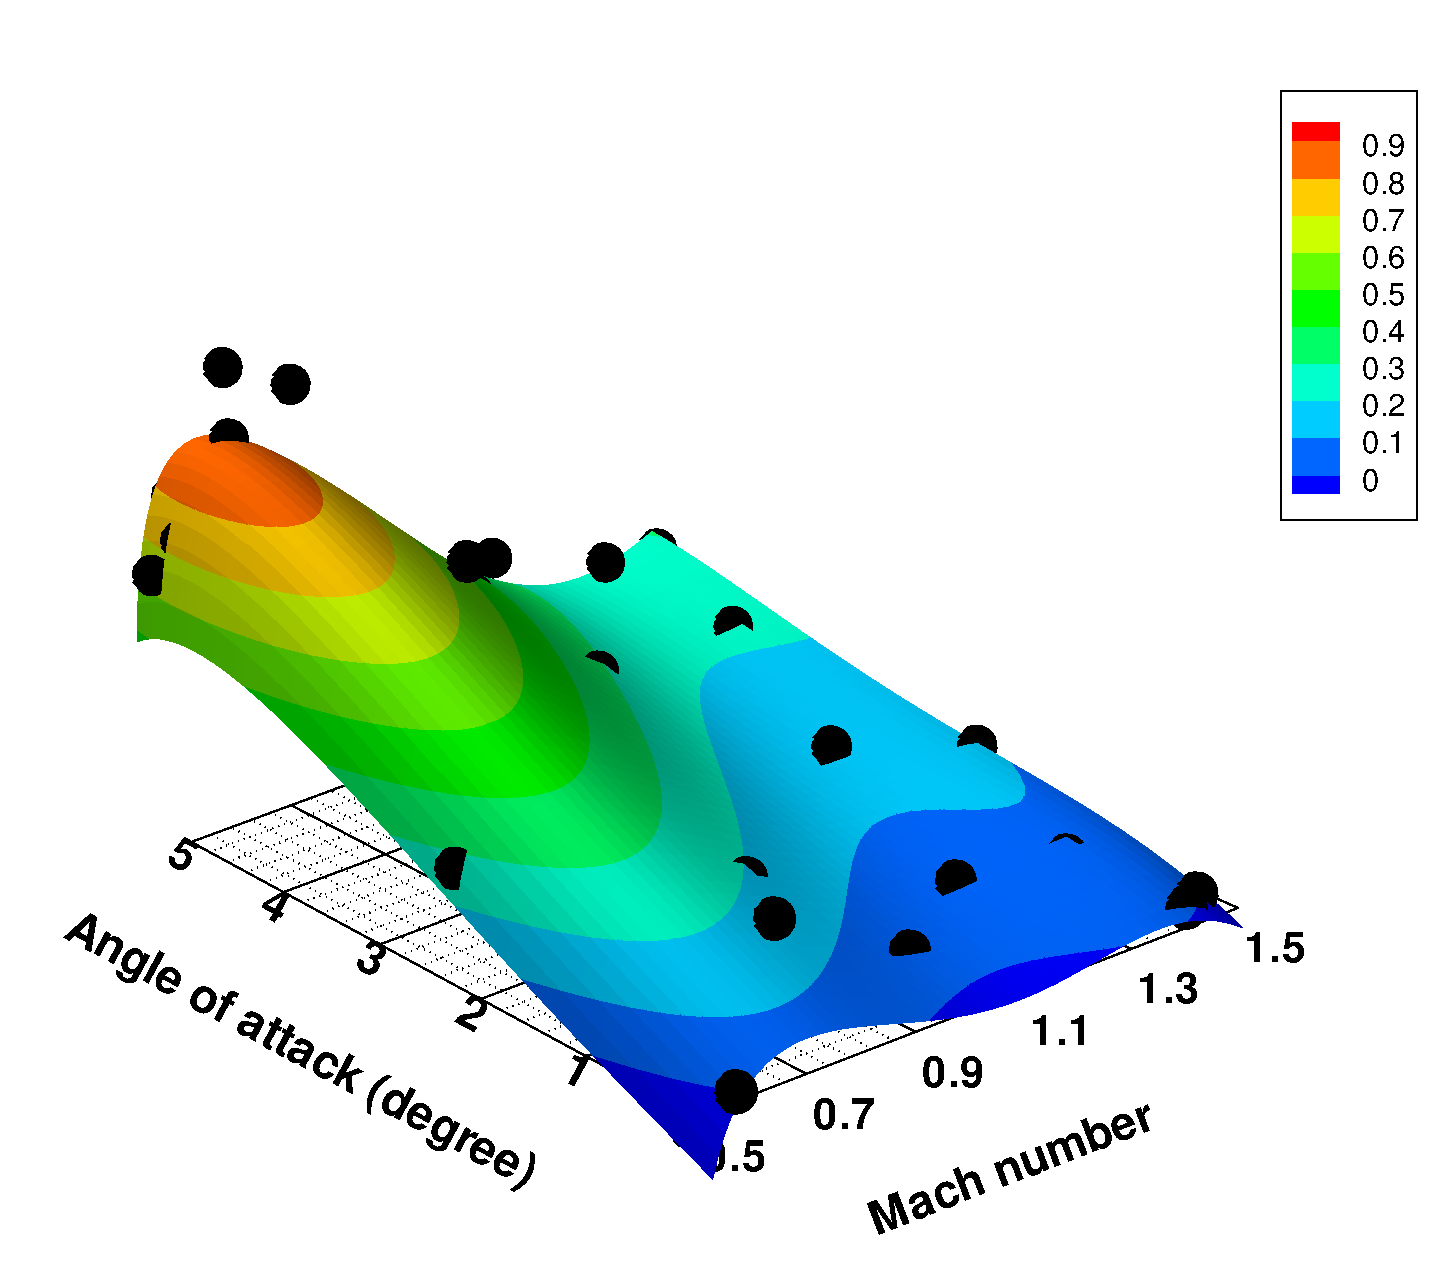
\includegraphics[width=1.0\textwidth]{liftpc30.eps} % \caption*{PC Lift}
\end{minipage}
\caption[Aerodynamic database of drag and lift coefficients with kriging and PCE.]{Contours of exact database (left), kriging (middle) and PCE (right) for drag (top) and lift coefficients (bottom) with 30 training points chosen with dynamic training point selection.}
\label{databaseplots}
\end{figure}


\subsection{Variable-Fidelity Kriging Results}

As mentioned in previous chapters, kriging supports the usage of both high- and low-fidelity training points~\cite{Han2012,Han2012b,Han2009,Han2010,Yamazaki2013,Yamazaki2012,Yamazaki2011b}.
The general idea is to combine trends from low-fidelity data (e.g., coarser meshes, less sophisticated models) with interpolations of high-fidelity data (e.g., finer meshes, better models, experimental data).
This approach can help to reduce the time taken to build an accurate surrogate model, since the low-fidelity data can be obtained much faster.
In this work a simple cokriging with cross-covariances between the low- and high-fidelity data is used~\cite{Yamazaki2013,Yamazaki2012}.
The low-fidelity data is calculated on a mesh with only 4,433 triangular elements (not shown), which is roughly four times cheaper to solve than the mesh shown in Figure~\ref{mesh} on which the high-fidelity data is calculated.

\begin{figure}[h!]
\centering
\begin{minipage}[b]{0.49\linewidth}
   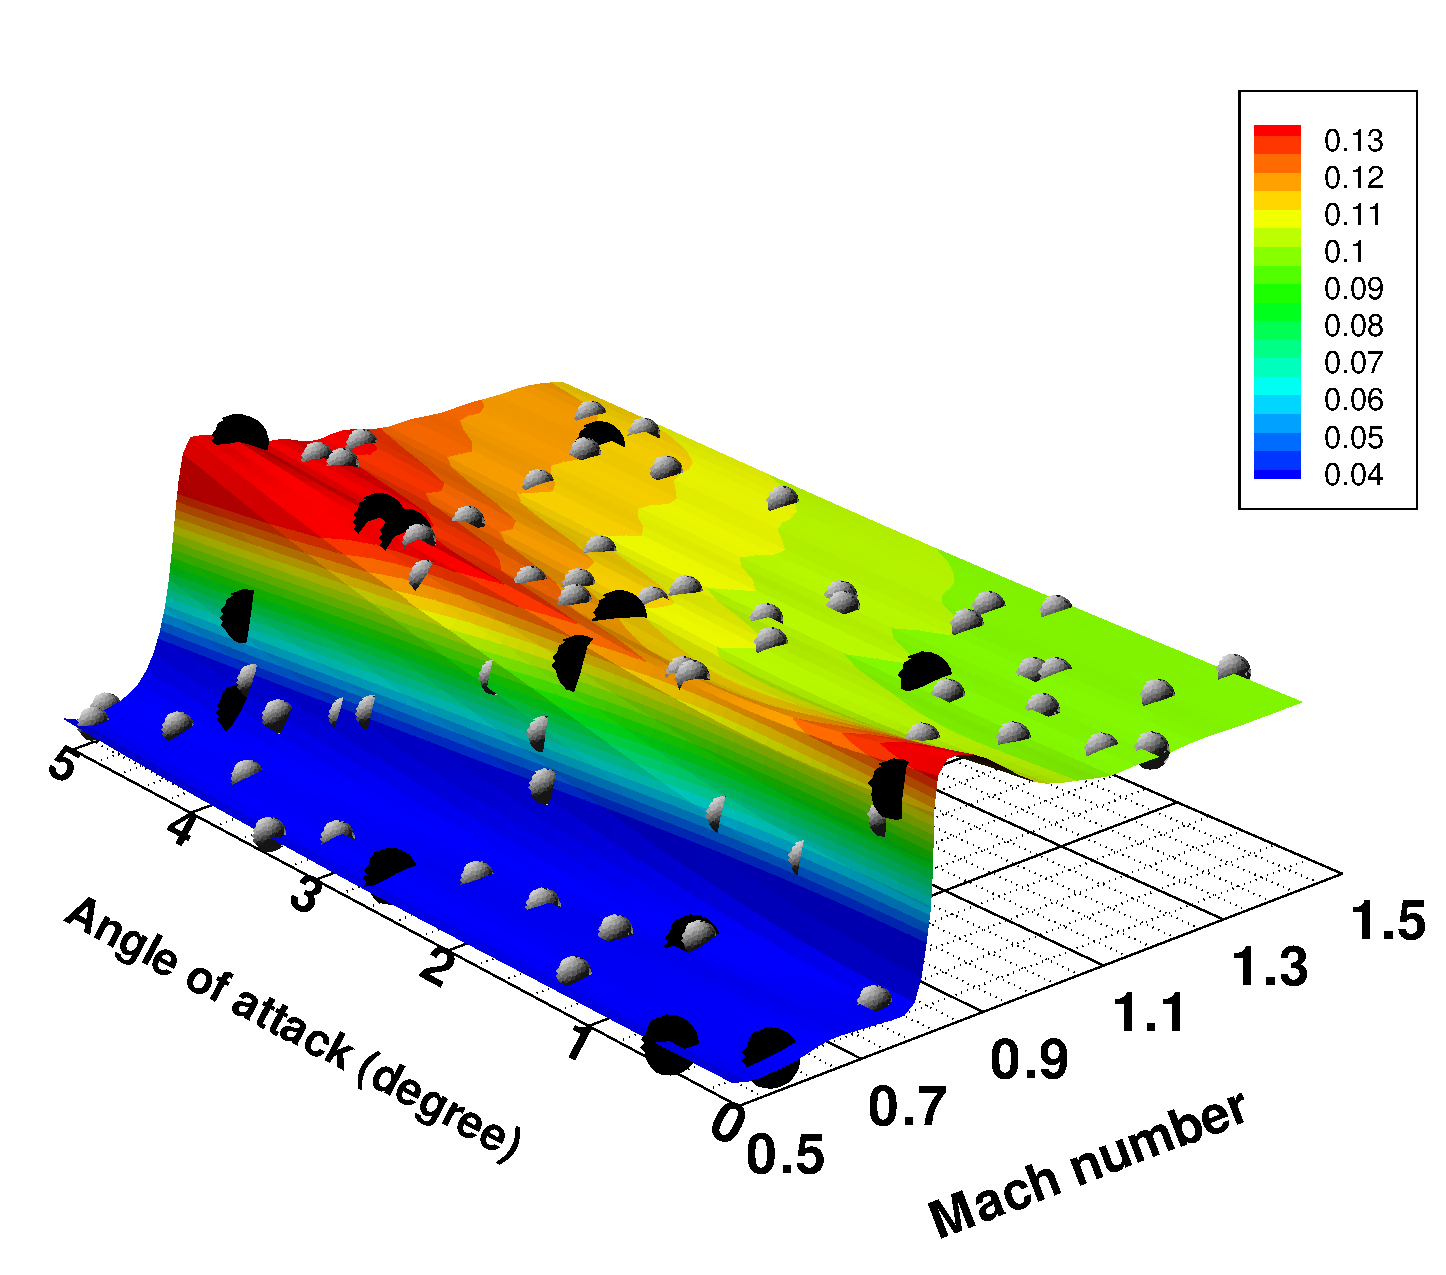
\includegraphics[width=1.0\textwidth]{krigdragh15l60.eps}
\end{minipage}
\begin{minipage}[b]{0.49\linewidth}
  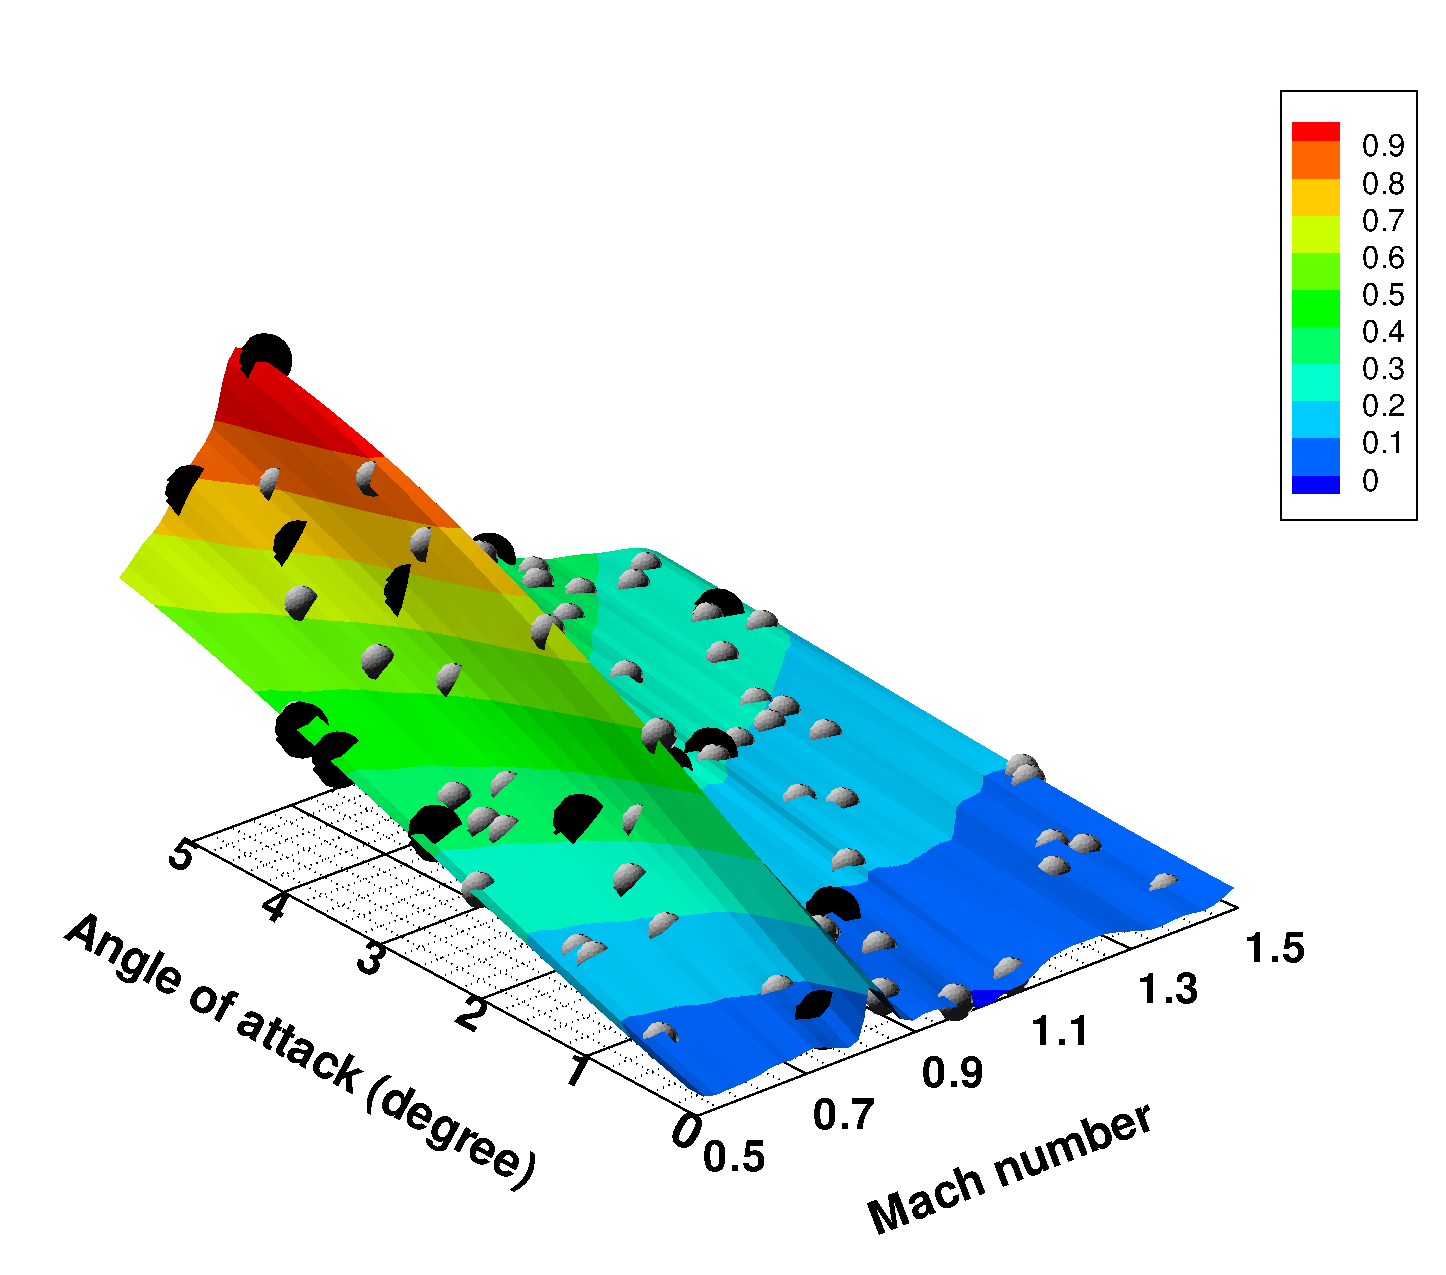
\includegraphics[width=1.0\textwidth]{kriglifth15l60.eps}
\end{minipage}
\caption[Aerodynamic database with variable-fidelity kriging.]{Kriging contour plots demonstrating the use of
  variable-fidelity data for drag (left) and lift (right) coefficients.}
\label{varfid}
\end{figure}


Figure~\ref{varfid} shows the variable-fidelity kriging contours for the drag and lift databases.  Here, $15$ high-fidelity and $60$ low-fidelity training
points were used in the construction of the kriging surrogate and the training point locations are shown as spheres,
where the dark spheres are high-fidelity training points picked dynamically and the smaller gray spheres are low-fidelity training points
picked via LHS. The overall computational cost is roughly equivalent to the construction of the kriging surrogate model using $30$ high-fidelity training points.
An improvement in the accuracy of the model can be noticed when using the variable-fidelity data by comparing Figures~\ref{databaseplots} and \ref{varfid} as well as from Table~\ref{tablekrig}, for roughly the same computational cost.
\begin{table}[h!]
\caption{RMSE comparisons for different kriging models.}
\medskip
\centering 
\scalebox{0.98}{\begin{tabular}{c c c}
\hline\hline
 {RMSE} & High-fidelity & Variable-fidelity \\
& (30 high-fidelity points) & ($15$ high-fidelity and $60$ low-fidelity points)\\
\hline\hline
\medskip
 Drag Coefficient \nom{$C_D$}{drag coefficient} & $0.39\times10^{-2}$  & $0.31\times10^{-2}$\\
 Lift Coefficient \nom{$C_L$}{lift coefficient} & $0.35\times10^{-1}$  & $0.18\times10^{-1}$\\[1ex]
\hline
\end{tabular}}
\label{tablekrig}
\end{table}
